\documentclass[10pt, a4paper]{article}

\usepackage{ctex}
\usepackage{xeCJK}
\usepackage{caption}
\usepackage{geometry}
\geometry{
    left = 0.6in,
    right = 0.6in,
    top = 0.8in,
    bottom = 1.0in
}
\usepackage{amssymb}
\usepackage{amsbsy}
\usepackage{amsmath}
\usepackage{xcolor}
\usepackage{mathrsfs}
\usepackage{graphicx}
\usepackage{pifont}
\usepackage{tasks}
\settasks{
    label = \Alph*. ,
    label-width = 16pt
}
\pagestyle{empty}

\newcommand{\Title}[3]{
    \begin{center}
        \Large \textbf{中国电子学会 #1~年~#2~月 Scratch~#3级考试}
    \end{center}
}
\newcommand{\TimeAndName}[1]{
    \begin{center}
        考试时间:~#1~ 分钟 \qquad\qquad\qquad\qquad 姓名:\underline{\quad\quad\quad\quad}
    \end{center}
}

\begin{document}
    \Title{2021}{6}{二} % 标题
    \TimeAndName{60} % 考试时间及姓名

    % 单选题
    \vspace{2mm}
    {\noindent\textbf{第一部分、单选题(共 25 题,每题 2 分,共50分.)}}
    \begin{enumerate}
        % 1
        \item 小明同学设计了一款游戏,其中一段程序如下图所示,下面这段程序可以实现哪项功能?(\qquad)
        \begin{tasks}(2)
            \task 在任何地方点击鼠标,角色都会移到鼠标位置
            \task 没有任何操作的时候角色会在舞台区域随机移动
            \task 按下空格键后,角色会在一秒内滑行到舞台中央
            \task 角色碰到黄色会说“恭喜获得胜利!”
        \end{tasks}

        % 2
        \item 小猫程序对应流程图和在舞台位置如下图所示,其中流程图中的红色与舞台上红色一样,请问小猫会说?(\qquad)
        \begin{tasks}(2)
            \task 碰到红色
            \task 没有碰到红色
            \task 先说“碰到红色”,再说“没有碰到红色”
            \task 先说“没有碰到红色”,再说“碰到红色”
        \end{tasks}

        \begin{figure}[htbp]
            \centering
            \begin{minipage}[t]{.2\textwidth}
                \centering
                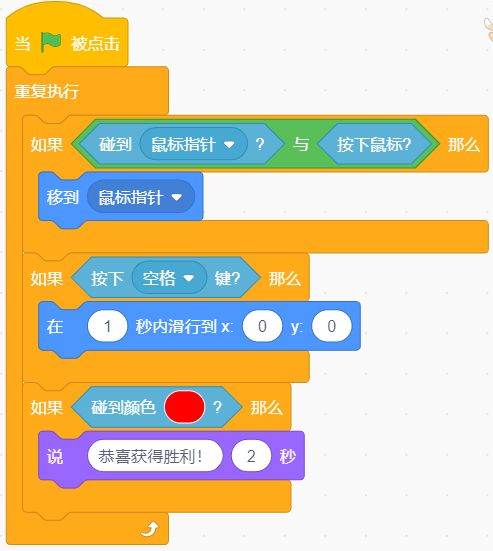
\includegraphics[width=1\textwidth]{1.png}
                \caption*{第1题}
            \end{minipage}
            \begin{minipage}[t]{.5\textwidth}
                \centering
                \begin{minipage}[t]{.45\textwidth}
                    \centering
                    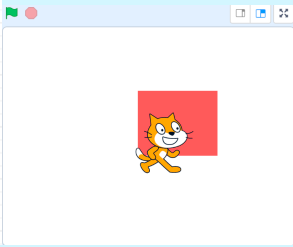
\includegraphics[width=\textwidth]{2-1.png}
                \end{minipage}
                \begin{minipage}[t]{.53\textwidth}
                    \centering
                    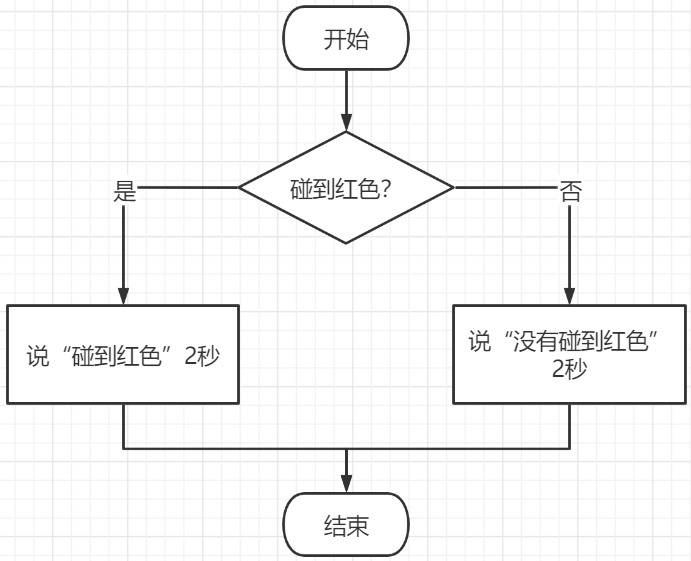
\includegraphics[width=\textwidth]{2-2.png}
                \end{minipage}
                \caption*{第2题}
            \end{minipage}
            \begin{minipage}[t]{.23\textwidth}
                \centering
                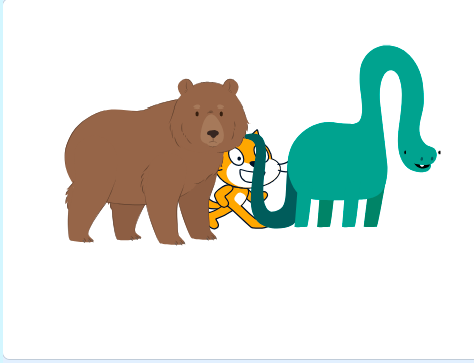
\includegraphics[width=\textwidth]{3.png}
                \caption*{第3题}
            \end{minipage}
        \end{figure}

        % 3
        \item 观察下图,如果想让小猫显示在熊和恐龙的最前面,使用下面哪个方法可以完成?(\qquad)
        \begin{tasks}(4)
            \task 将小猫“移到最前面”
            \task 将小猫“移到最后面”
            \task 将小熊“移到最后面”
            \task 将恐龙“移到最后面”
        \end{tasks}

        % 4
        \item 默认小猫角色现在在舞台的中心(坐标系原点)位置,如果想让它往右上角移动,下面哪个积木是正确的?(\qquad)
        \begin{tasks}(4)
            \task 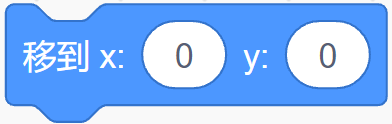
\includegraphics[width=.15\textwidth]{4a.png}
            \task 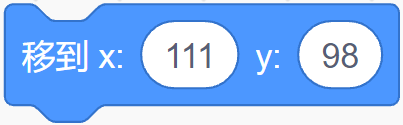
\includegraphics[width=.15\textwidth]{4b.png}
            \task 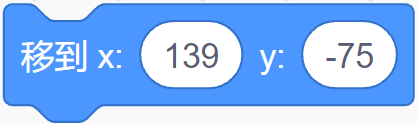
\includegraphics[width=.15\textwidth]{4c.png}
            \task 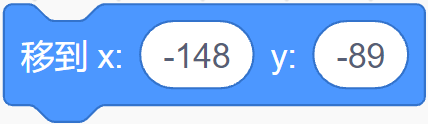
\includegraphics[width=.15\textwidth]{4d.png}
        \end{tasks}

        % 5
        \item 下面程序运行的结果是?(\qquad)
        
        \begin{minipage}{.3\textwidth}
            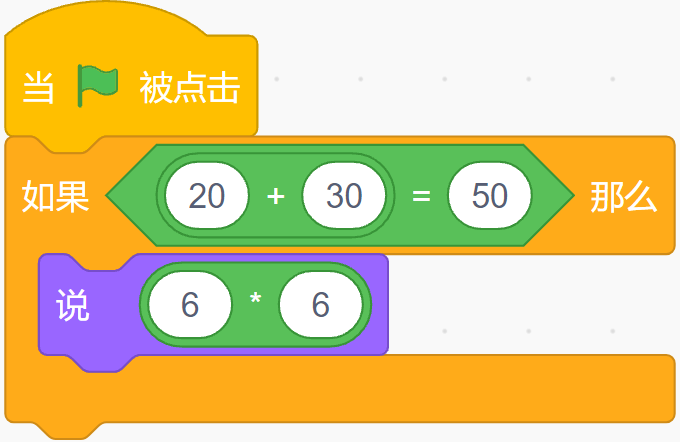
\includegraphics[width=.6\textwidth]{5.png}
        \end{minipage}
        \begin{minipage}{.6\textwidth}
            \begin{tasks}(2)
                \task 无结果
                \task 说“6*6”
                \task 说“50”
                \task 说“36”
            \end{tasks}
        \end{minipage}

        % 6
        \item 下面哪个选项能计算出四则运算$2021-8\times (8+8)$的结果是?(\qquad)
        \begin{tasks}(4)
            \task 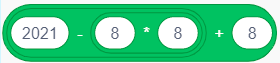
\includegraphics[width=.18\textwidth]{6a.png}
            \task 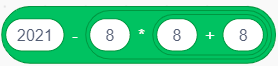
\includegraphics[width=.18\textwidth]{6b.png}
            \task 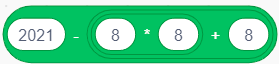
\includegraphics[width=.18\textwidth]{6c.png}
            \task 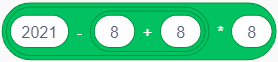
\includegraphics[width=.18\textwidth]{6d.png}
        \end{tasks}

        % 7
        \item 想让角色一直在舞台上移动,应使用下面哪个选项的积木?(\qquad)
        \begin{tasks}(4)
            \task 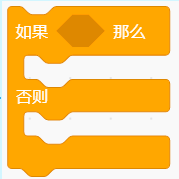
\includegraphics[width=.1\textwidth]{7a.png}
            \task 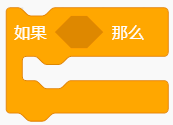
\includegraphics[width=.12\textwidth]{7b.png}
            \task 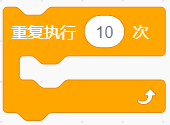
\includegraphics[width=.12\textwidth]{7c.png}
            \task 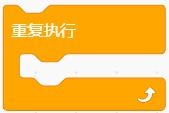
\includegraphics[width=.12\textwidth]{7d.png}
        \end{tasks}

       % 8
       \item 小明、小刚、小军和老师外出踏青,由于天气炎热,老师给学生们买了几瓶饮料,买来后,三位小朋友对饮料数量有如下猜测:小明说:饮料数量小于3瓶小刚说:饮料数量不小于5瓶小军说:我们每个人可以喝2瓶结果是三人都猜错了,老师把饮料平均分给三人,自己也喝了一瓶后没有剩余,那老师一共买了几瓶饮料呢?(\qquad)
       \begin{tasks}(4)
           \task 3
           \task 4
           \task 5
           \task 6
       \end{tasks}

        % 9
        \item 默认小猫,初始位置在舞台中心,面向右,下面哪个程序能够绘制出一个四条边粗细都不相同的四边形?(\qquad)
        \begin{tasks}(4)
            \task 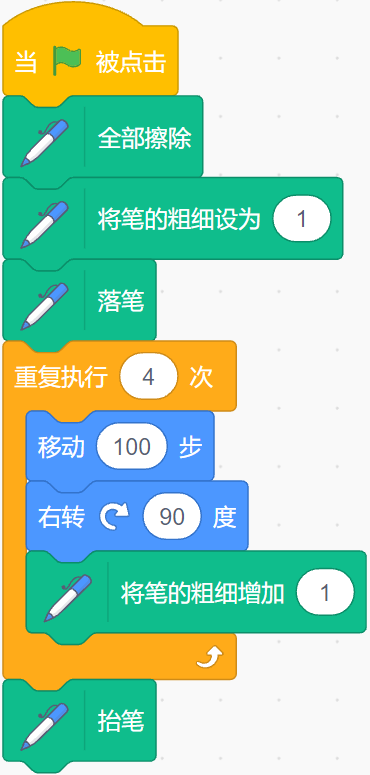
\includegraphics[width=.12\textwidth]{9a.png}
            \task 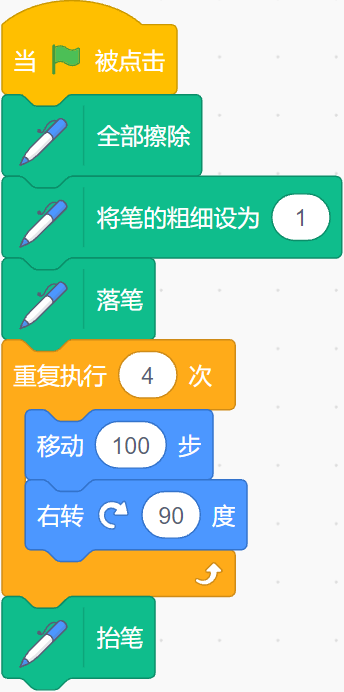
\includegraphics[width=.125\textwidth]{9b.png}
            \task 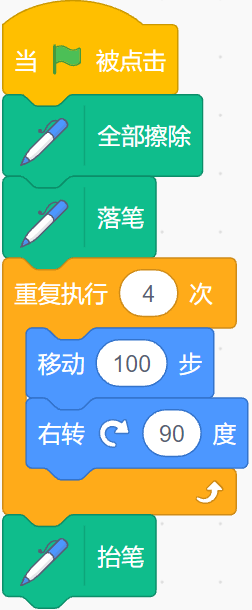
\includegraphics[width=.105\textwidth]{9c.png}
            \task 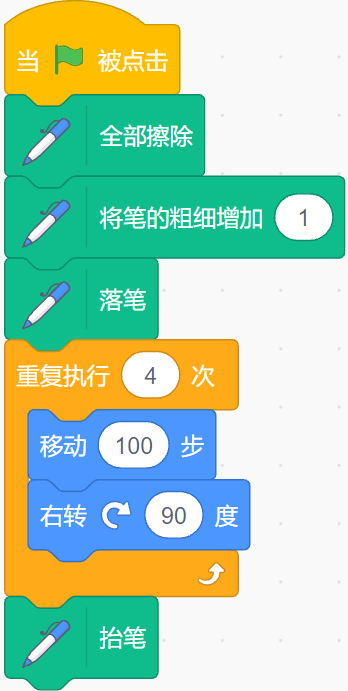
\includegraphics[width=.13\textwidth]{9d.png}
        \end{tasks}

        % 10
        \item 舞台有多个不同的背景,执行下面程序后说法正确的是?(\qquad)
        \begin{tasks}(2)
            \task 程序用到了循环语句
            \task 执行完程序后,角色会说“你好!”
            \task 执行完程序后,会变换舞台背景
            \task 程序执行完后,角色说“你好!”,舞台变换背景
        \end{tasks}

        % 11
        \item 舞台如下图所示,下面哪个选项在不改变参数的情况下,能让小猫不见了?(\qquad)
        \begin{tasks}(4)
            \task 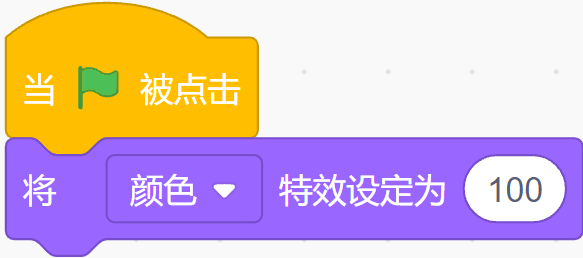
\includegraphics[width=.16\textwidth]{11a.png}
            \task 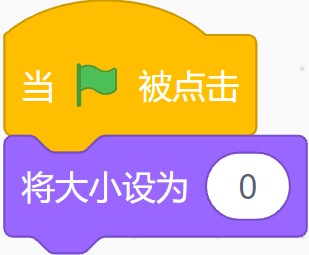
\includegraphics[width=.08\textwidth]{11b.png}
            \task 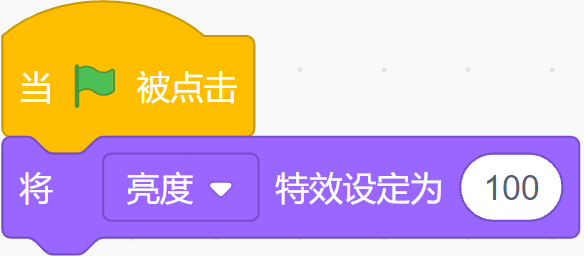
\includegraphics[width=.16\textwidth]{11c.png}
            \task 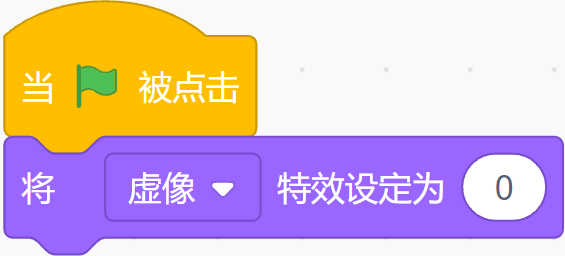
\includegraphics[width=.16\textwidth]{11d.png}
        \end{tasks}

        % 12
        \item 执行下图程序后,角色$x$坐标是?(\qquad)
        \begin{tasks}(4)
            \task 20
            \task 30
            \task 100
            \task 50
        \end{tasks}

        \begin{figure}[htbp]
            \centering
            \begin{minipage}[t]{.16\textwidth}
                \centering
                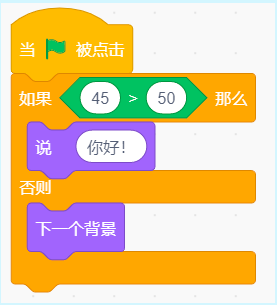
\includegraphics[width=\textwidth]{10.png}
                \caption*{第10题}
            \end{minipage}
            \begin{minipage}[t]{.22\textwidth}
                \centering
                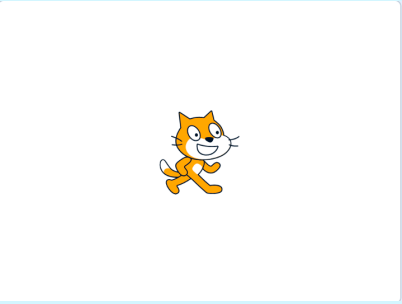
\includegraphics[width=\textwidth]{11.png}
                \caption*{第11题}
            \end{minipage}
            \begin{minipage}[t]{.13\textwidth}
                \centering
                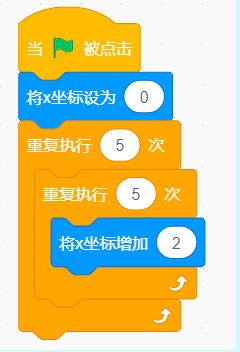
\includegraphics[width=\textwidth]{12.png}
                \caption*{第12题}
            \end{minipage}
            \begin{minipage}[t]{.35\textwidth}
                \centering
                \begin{minipage}[t]{.4\textwidth}
                    \centering
                    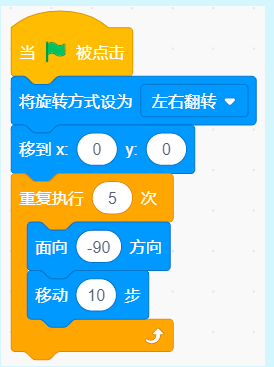
\includegraphics[width=\textwidth]{14-1.png}
                \end{minipage}
                \begin{minipage}[t]{.5\textwidth}
                    \centering
                    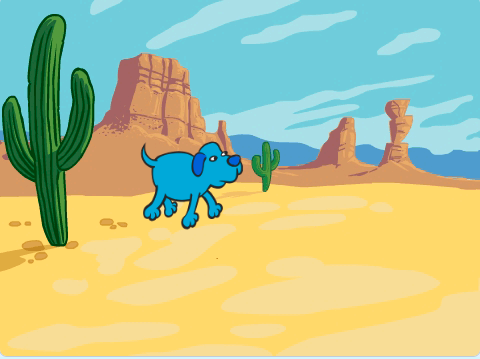
\includegraphics[width=\textwidth]{14-2.png}
                \end{minipage}
                \caption*{第14题}
            \end{minipage}
        \end{figure}

        % 13
        \item 把图形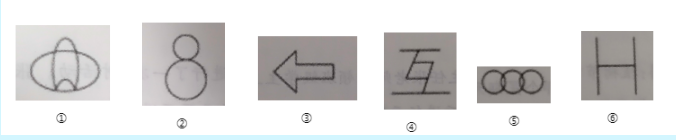
\includegraphics[width=.3\textwidth]{13.png}分为两类,使每一类图形都有各自的共同特征或规律,分类正确的一项是?(\qquad)
        \begin{tasks}(4)
            \task \ding{172}\ding{175}\ding{177},\ding{173}\ding{174}\ding{176}
            \task \ding{172}\ding{174}\ding{175},\ding{173}\ding{176}\ding{177}
            \task \ding{172}\ding{174}\ding{176},\ding{173}\ding{175}\ding{177}
            \task \ding{172}\ding{173}\ding{176},\ding{174}\ding{175}\ding{177}
        \end{tasks}

        % 14
        \item 如上图所示,下列程序执行后,角色一共移动了多少步?(\qquad)
        \begin{tasks}(4)
            \task 向右移动50步
            \task 向左移动50步
            \task 向左移动10步
            \task 向右移动10步
        \end{tasks}

        % 15
        \item 正方形的一条边长是2,下面哪个程序能正确计算出正方形的周长的是?(\qquad)
        \begin{tasks}(4)
            \task 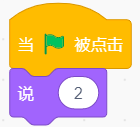
\includegraphics[width=.08\textwidth]{15a.png}
            \task 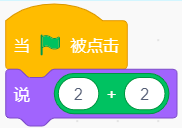
\includegraphics[width=.1\textwidth]{15b.png}
            \task 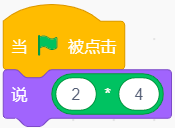
\includegraphics[width=.1\textwidth]{15c.png}
            \task 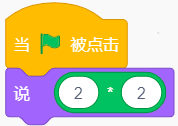
\includegraphics[width=.1\textwidth]{15d.png}
        \end{tasks}

        % 16
        \item 下面这段程序用来绘制图形,猜一猜它画出的是什么形状?(\qquad)
        \begin{tasks}(4)
            \task 椭圆
            \task 正方形
            \task 圆形
            \task 三角形
        \end{tasks}

        \begin{figure}[htbp]
            \centering
            \begin{minipage}[t]{.1\textwidth}
                \centering
                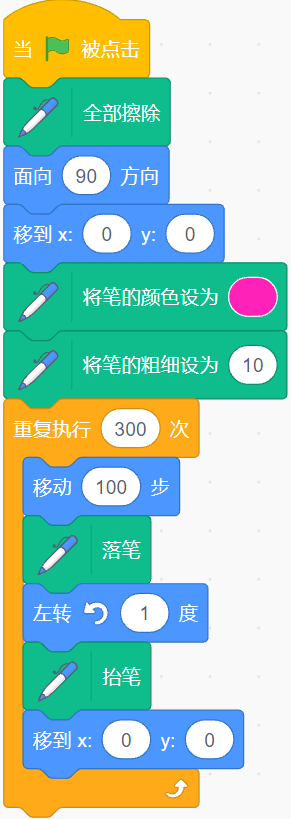
\includegraphics[width=\textwidth]{16.png}
                \caption*{第16题}
            \end{minipage}
            \begin{minipage}[t]{.18\textwidth}
                \centering
                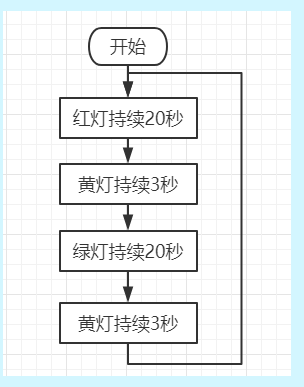
\includegraphics[width=\textwidth]{17.png}
                \caption*{第17题}
            \end{minipage}
            \begin{minipage}[t]{.2\textwidth}
                \centering
                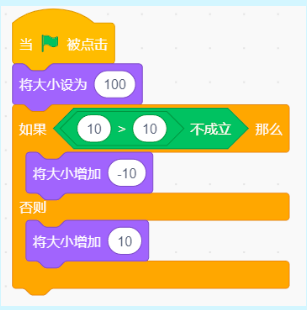
\includegraphics[width=\textwidth]{18.png}
                \caption*{第18题}
            \end{minipage}
            \begin{minipage}[t]{.18\textwidth}
                \centering
                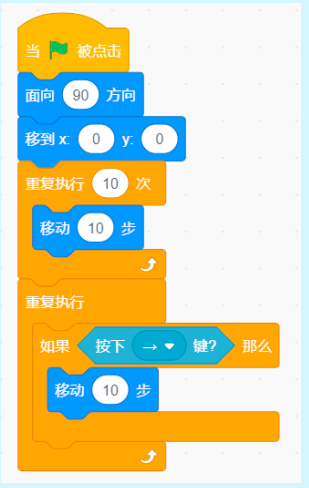
\includegraphics[width=\textwidth]{20.png}
                \caption*{第20题}
            \end{minipage}
        \end{figure}

        % 17
        \item 红绿灯程序流程图如上图所示,它是属于那种结构流程图?(\qquad)
        \begin{tasks}(4)
            \task 顺序结构流程图
            \task 循环结构流程图
            \task 选择结构流程图
            \task 语言结构流程图
        \end{tasks}

        % 18
        \item 运行上面程序后角色大小为?(\qquad)
        \begin{tasks}(4)
            \task 10
            \task 90
            \task 100
            \task 110
        \end{tasks}

        % 19
        \item 在声音编辑面板中
\includegraphics[width=.4\textwidth]{19.png}可以设置下图中的声音特效,不包括下面哪个选项?(\qquad)
        \begin{tasks}(4)
            \task 渐强
            \task 反转
            \task 机械化
            \task 重音
        \end{tasks}

        % 20
        \item 运行上面程序,说法正确的是?(\qquad)
        \begin{tasks}
            \task 点击绿旗角色会移到舞台中央,直到按下$\to$键角色才向右移动10步
            \task 点击绿旗角色会移到舞台中央,按下$\to$键角色向左移动10步
            \task 点击绿旗角色会移到舞台中央,向右移动100步,再按下一次$\to$键角色向右移动10步
            \task 点击绿旗角色会移到舞台中央,角色向右移动10步,再按下$\to$键角色向左移动10步
        \end{tasks}

        % 21
        \item 下列数学运算中,结果一定为2021的是?(\qquad)
        \begin{tasks}(4)
            \task 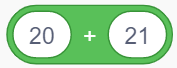
\includegraphics[width=.12\textwidth]{21a.png}
            \task 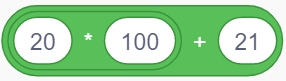
\includegraphics[width=.15\textwidth]{21b.png}
            \task 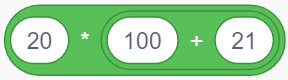
\includegraphics[width=.15\textwidth]{21c.png}
            \task 
\includegraphics[width=.15\textwidth]{21d.png}
        \end{tasks}

        % 22
        \item 找规律填数字是一种很有趣的游戏,特别锻炼观察和思维能力,填入数列“1、3、7、15、31、(\quad)”空缺处的数字,下列选项正确的是?(\qquad)
        \begin{tasks}(4)
            \task 35
            \task 40
            \task 62
            \task 63
        \end{tasks}

        % 23
        \item 默认小猫角色,初始位置在舞台中心,面向右,执行下面程序,说法正确的是?(\qquad)
        \begin{tasks}(2)
            \task 程序会一直执行下去
            \task 角色在移动过程中不会切换造型
            \task 角色会一直移动到舞台边缘然后停下来
            \task 角色碰到舞台边缘后就不切换造型了
        \end{tasks}

        % 24
        \item 动画片正在播放音乐,下面哪个积木可以让音乐停止播放?(\qquad)
        \begin{tasks}(4)
            \task 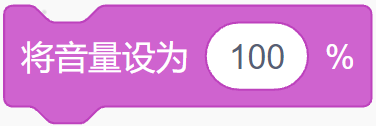
\includegraphics[width=.12\textwidth]{24a.png}
            \task 
\includegraphics[width=.18\textwidth]{24b.png}
            \task 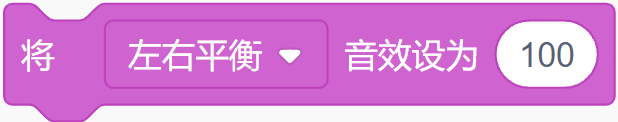
\includegraphics[width=.18\textwidth]{24c.png}
            \task 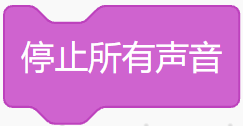
\includegraphics[width=.08\textwidth]{24d.png}
        \end{tasks}

        % 25
        \item 下面哪个积木的运算结果为true?(\qquad)
        \begin{tasks}(4)
            \task 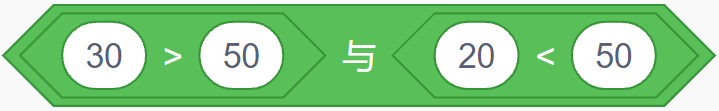
\includegraphics[width=.18\textwidth]{25a.png}
            \task 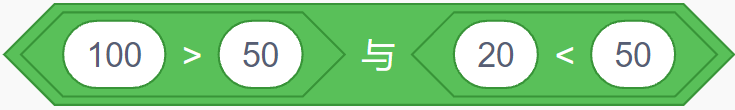
\includegraphics[width=.18\textwidth]{25b.png}
            \task \includegraphics[width=.18\textwidth]{25c.png}
            \task \includegraphics[width=.18\textwidth]{25d.png}
        \end{tasks}

        \begin{figure}[htbp]
            \centering
            \begin{minipage}[t]{.2\textwidth}
                \centering
                \includegraphics[width=\textwidth]{23.png}
                \caption*{第23题}
            \end{minipage}
            \begin{minipage}[t]{.1\textwidth}
                \centering
                \includegraphics[width=\textwidth]{26.png}
                \caption*{第26题}
            \end{minipage}
            \begin{minipage}[t]{.15\textwidth}
                \centering
                \includegraphics[width=\textwidth]{28.png}
                \caption*{第28题}
            \end{minipage}
        \end{figure}
    \end{enumerate}

    % 判断题
    {\noindent\textbf{第二部分、判断题(共 10 题,每题 2 分,共20分.)}}
    \begin{enumerate}
        \setcounter{enumi}{25}
        % 26
        \item 执行上面程序后,舞台上有一条虚线.(\qquad)

        %27
        \item 程序\includegraphics[width=.18\textwidth]{27.png}结果为$-5$.(\qquad)

        %28
        \item 编程实现键盘输入的数大于50,角色大小就增加10;否则角色右转15度,会用到上面积木.(\qquad)
  
        %29
        \item 默认小猫角色,执行下面程序,只有当角色碰到舞台边缘时才会停止移动.(\qquad)
        
        %30
        \item 积木\includegraphics[width=.2\textwidth]{30.png}的结果为3.(\qquad)
        
        %31
        \item 点击绿旗后,每次按下空格键时,角色大小一定会减少50.(\qquad)
        
        \begin{figure}[htbp]
            \centering
            \begin{minipage}[t]{.18\textwidth}
                \centering
                \includegraphics[width=\textwidth]{29.png}
                \caption*{第29题}
            \end{minipage}
            \begin{minipage}[t]{.38\textwidth}
                \centering
                \includegraphics[width=\textwidth]{31.png}
                \caption*{第31题}
            \end{minipage}
            \begin{minipage}[t]{.15\textwidth}
                \centering
                \includegraphics[width=\textwidth]{33.png}
                \caption*{第33题}
            \end{minipage}
            \begin{minipage}[t]{.13\textwidth}
                \centering
                \includegraphics[width=\textwidth]{34.png}
                \caption*{第34题}
            \end{minipage}
        \end{figure}
        
        %32
        \item 画笔模块中的“落笔”可以在舞台上印出一个与角色相同的图案.(\qquad)
                
        %33
        \item 执行上面程序,角色会在舞台上四处移动,碰到边缘反弹.(\qquad)
                
        %34
        \item 执行上面程序,角色会重复执行移到鼠标指针位置.(\qquad)
                
        %35
        \item Scratch中对角色进行复制时,产生的新的角色,修改新角色的程序也会修改之前被复制的角色的程序.(\qquad)
    \end{enumerate}

    \newpage
    {\noindent \textbf{第三部分、编程题(共 2 题,共30分.)}}
    \begin{enumerate}
        \setcounter{enumi}{35}
        
        % 36
        \item 绘制五彩缤纷的多瓣花:
        \begin{figure}[htbp]
            \begin{minipage}{.6\textwidth}
                1. 准备工作
                \begin{tasks}[label = (\arabic*)]
                    \task 删除默认的小猫角色,绘制角色,一片花瓣;
                    \task 采留默认白色背景.
                \end{tasks}
                2. 功能实现
                \begin{tasks}[label = (\arabic*)]
                    \task 按下数字5清空屏幕,移到随机位置,画出5个花瓣的花;
                    \task 按下数字6清空屏幕,移到随机位置,画出6个花瓣的花;
                    \task 按下数字8清空屏幕,移到随机位置,画出8个花瓣的花;

                    【注意有个花心,如上图所示】

                    \task 花瓣的颜色不相同;
                    \task 按下数字0清空屏幕.
                \end{tasks}
            \end{minipage}
            \begin{minipage}{.37\textwidth}
                \centering
                \includegraphics[width=\textwidth]{36.png}
            \end{minipage}
        \end{figure}

        % 37
        \item 小瓢虫找妈妈:
        \begin{figure}[htbp]
            \begin{minipage}{.6\textwidth}
                1. 准备工作
                \begin{tasks}[label = (\arabic*)]
                    \task 删除默认的小猫角色,添加“ladybug1”作为小飘虫角色;
                    \task 添加"ladybug2"作为飘虫妈妈角色;
                    \task 绘制“轨迹”角色即为飘虫妈妈留下的轨迹;
                    \task 添加背景"Blue Sky".
                \end{tasks}
                2. 功能实现
                \begin{tasks}[label = (\arabic*)]
                    \task 点击绿旗,小飘虫舞台左下方,在轨迹的一头,飘虫妈妈在舞台右上方,在轨迹的另外一头;
                    \task 小飘虫沿着飘虫妈妈留下的轨迹走到飘虫妈妈的身边(提示:可以给小飘虫的两个触须涂成不同颜色,作为探测器,两个触须碰到中间轨迹颜色,会调节左右旋转);
                    \task 小飘虫碰到飘虫妈妈停下来.
                \end{tasks}
            \end{minipage}
            \begin{minipage}{.37\textwidth}
                \centering
                \includegraphics[width=\textwidth]{37.png}
            \end{minipage}
        \end{figure}
    \end{enumerate}
\end{document}